
\section{Simulation of the MPPT algorithm} \label{MPPTSimulation}

The results obtained in simulation for the previously explained P\&O algorithm will be shown in this section. First, the results corresponding to the PV panel model will be evaluated without connecting it to the DC-DC converter. Once the model for the PV panel is validated, the results obtained for the complete system will be analyzed in order to show the performance of the MPPT algorithm under different environmental conditions and resistive loads \todo{Confirm with the supervisors if resistive load or voltage source}.  

\subsection{Model of the PV panel}

This section shows the model and the results obtained from a commercial solar panel selected for the development of this project. The PV panel which will be utilized for the test of the MPPT is \textit{Suntech STP300-24/Vd} \todo{Ref to the datasheet of the panel. Remember to delete the old one. Stef}. As a result of the PV panel's model, the characteristic curves of the panel will be presented showing its behavior under variations in irradiance and temperature.

There are different modeling techniques for a solar panel, being the most common method based on the equivalent circuit of a solar cell shown in figure \ref{fig:eq_circuit_PVcell} \todo{consider rephrasing. AT}. It is observed that the model of the solar cell can be represented as a current source connected in antiparallel with an ideal p-n junction diode \todo{wouldn't all the current flow through the diode? AT}. In addition, to model the non-linear behaviour of the solar panel I-V curve the equivalent series and parallel resistance ($R_{s}$ and $R_{p}$) are inserted.


\begin{figure}[H]
	\begin{center}
		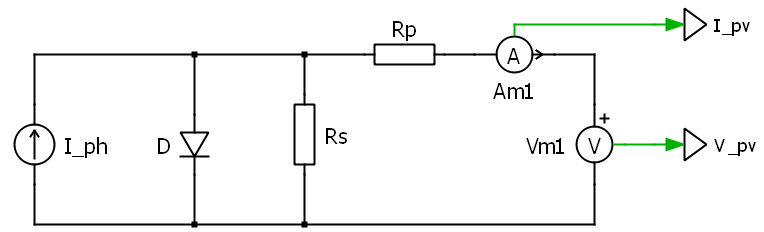
\includegraphics[width=0.8\textwidth]{../Pictures/schematic_pv_cell}
		\caption{Equivalent circuit of a PV cell.}
		\label{fig:eq_circuit_PVcell} 
	\end{center}	
\end{figure}

The mathematical equation that describes the equivalent circuit of the solar cell is presented in equation \ref{eq:pv_cell} \todo{REF to "Evaluation of main MPPT techniques... Stef} where $I_{pv}$ is the current output of the panel, $I_{ph}$ is the photogenerated current, the second term is the current drop in the diode and the last term is the current drop in the series resistance \todo{is current drop a thing? current flow or voltage drop i would say. AT}. 

\begin{equation} \label{eq:pv_cell}
I_{pv} = I_{ph} - I_{o} \cdot \left[ e^{\left({\dfrac{V_{pv} + R_s\cdot I_{pv}}{a \cdot V_{t}}}\right)}  - 1 \right]  - \dfrac{V_{pv} + R_{s}\cdot I_{pv}}{R_{p}}
\end{equation}

In the second term $I_{o}$ is the saturation current of the diode, $a$ is the p-n junction quality factor  and $V_{t}$ is the thermal voltage defined by

\begin{equation} 
V_{t}=\dfrac{N_{s}\cdot K\cdot T}{q} 
\end{equation}

where $N_{s}$ is the number of series connected cells (in this case 72), K is the Boltzmann constant ($1.38 \cdot 10^{-23} J/K$), T is the temperature in kelvins and q is the electrical charge ($1.6 \cdot 10^{-19} C$).

However, as the focus of this project is not the modelling of the PV panel, the value of the PV panel's parameters such as $R_{s}$, $R_{p}$ and $a$ required for the model will be taken from the corresponding PV array block for the selected panel available in \textit{Simulink}. All the values for the PV panel's electrical parameters corresponding to Standard Test Conditions (STC) are shown in table \ref{el_charact_PV_panel_Suntech}. The STC test is carried out at a solar cell's temperature of $25^\circ$C and at a solar irradiance of 1000 $W/ m^2$ \cite{handbook}.

\begin{table}[H]
	\centering
	\begin{tabular}{|p{8cm}|>{\centering}p{6cm}|}
		\hline
		\rowcolor{lightgray}\multicolumn{2}{|l|}{ \textbf{Electrical characteristics under Standard Test Conditions (STC)}} 
		\\ \hline
		Maximum power ($P_{max}$) & 300 [W]  \tabularnewline \hline
		Optimum Operating Voltage ($V_{mpp}$) & 36.9 [V]  \tabularnewline \hline
		Optimum Operating Current ($I_{mpp}$) & 8.14 [A]  \tabularnewline \hline
		Open Circuit Voltage ($V_{oc}$) &  45 [V] \tabularnewline \hline
		Short Circuit Current ($I_{sc}$) & 8.67 [A]  \tabularnewline \hline
		Module Efficiency ($\eta$) & 15.5 \%  \tabularnewline \hline
		Operating Module Temperature & -40$\dec$C to +85$\dec$C \tabularnewline \hline
		Series Resistance ($R_{s}$) & 0.266 [$\Omega$] \tabularnewline \hline
		Parallel Resistance ($R_{p}$) & 665.2 [$\Omega$] \tabularnewline \hline
		P-n junction quality factor ($a$) & 1.1098 \tabularnewline \hline
	\end{tabular}
	\caption{Electrical characteristics PV module \textit{Suntech STP300-24/Vd} \cite{PV_panel}.}\todo{Modify in the bibliography the reference to the datasheet of the panel}
	\label{el_charact_PV_panel_Suntech}
\end{table}

Using the aforementioned model of the PV panel, it is possible to obtain the characteristic curves of the panel. Figures \ref{fig:PVcurves_T25} and \ref{fig:IVcurves_T25} show the P-V and I-V curves of the solar panel with constant cell temperature ($T=25\dec C$) and varying the level of irradiance. 
As expected, the lower the level of irradiance the maximum power that the panel is capable of generating decreases. It can be validated that under STC the values for the optimal operating voltage and current from table \ref{el_charact_PV_panel_Suntech}  correspond to the values obtained in simulation. It is observed that a change in irradiance has as a consequence a high variation in $I_{mpp}$ but the optimal voltage $V_{mpp}$ does not reflect a significant variation. 

\begin{figure}[H]
	\begin{center}
		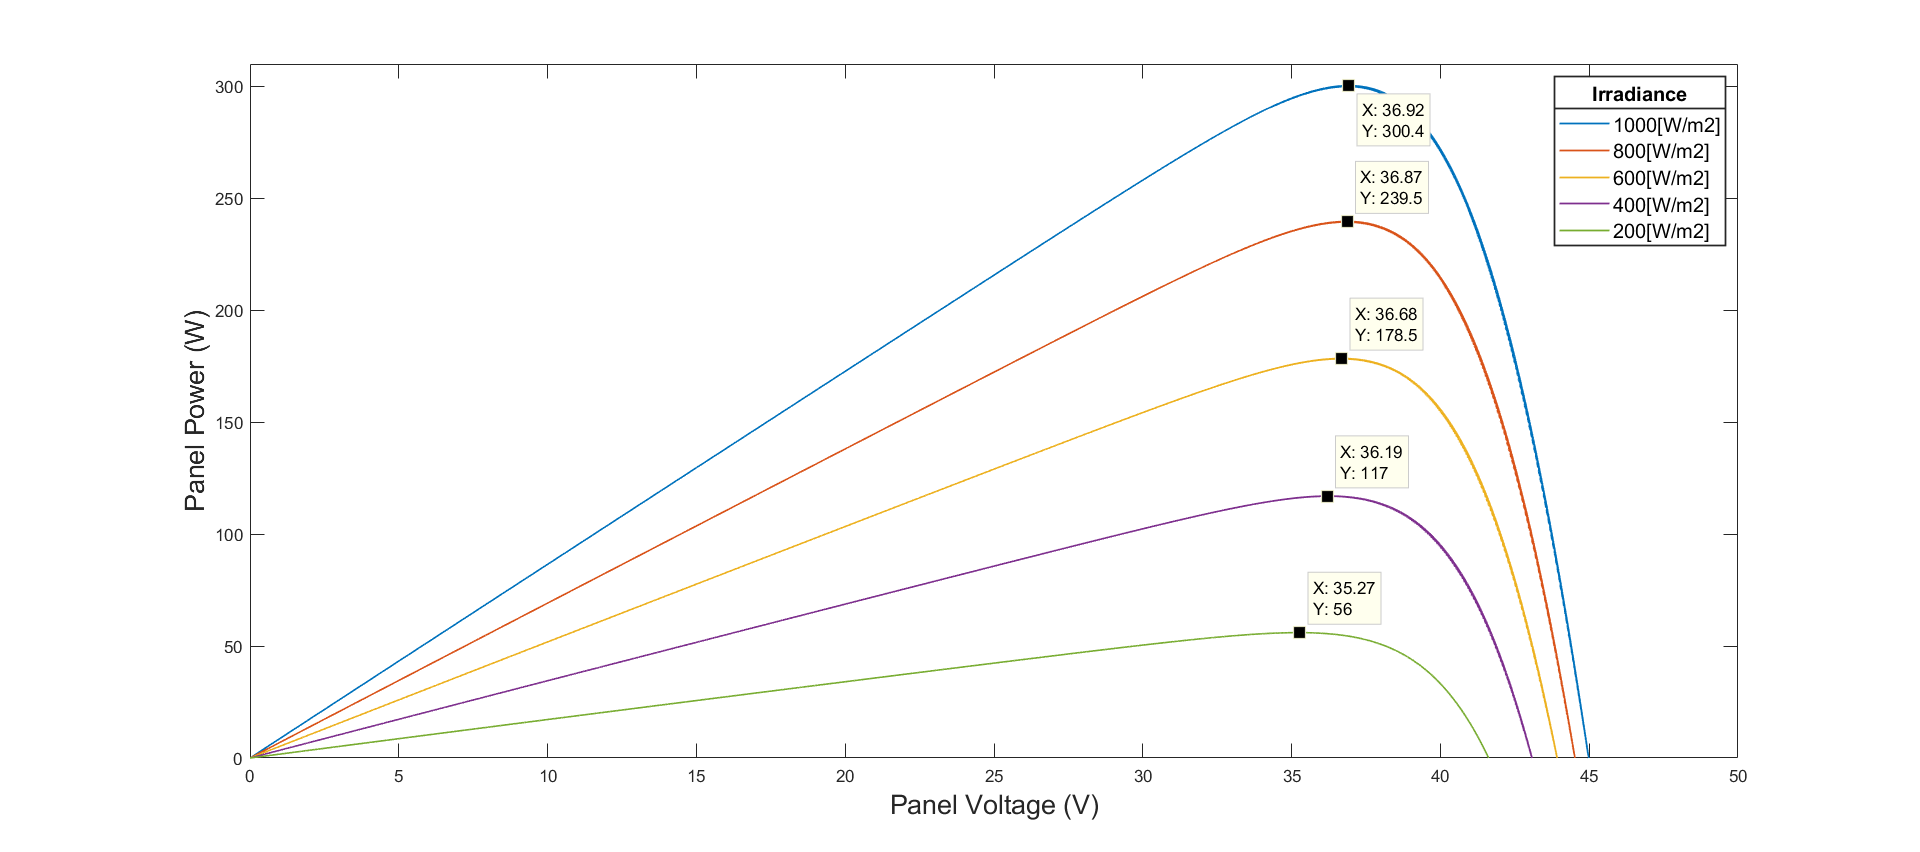
\includegraphics[width=0.83\textwidth]{../Pictures/PV_curves_T25degrees}
		\caption{P-V curves for constant temperature (25$\dec$C) and change in irradiance.}
		\label{fig:PVcurves_T25} 
	\end{center}	
\end{figure}

\begin{figure}[H]
	\begin{center}
		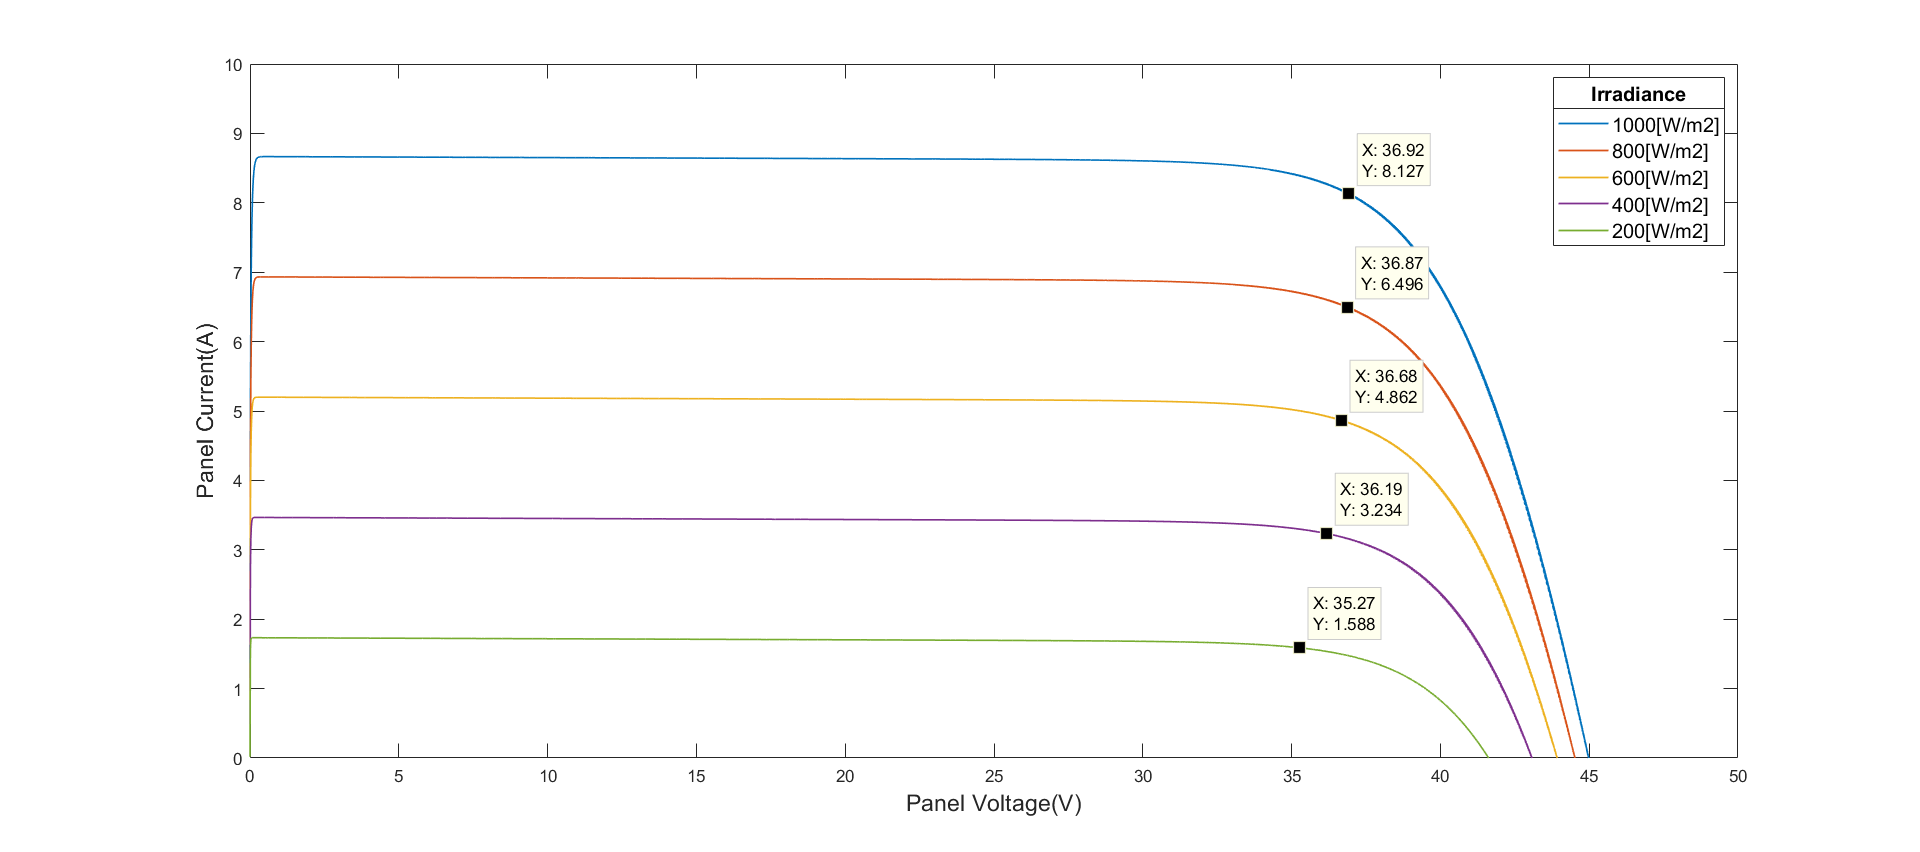
\includegraphics[width=0.83\textwidth]{../Pictures/IV_curves_T25degrees}
		\caption{I-V curves for constant temperature (25$\dec$C) and change in irradiance.}
		\label{fig:IVcurves_T25} 
	\end{center}	
\end{figure}

On the other hand, figures \ref{fig:PVcurves_Irr1000} and \ref{fig:IVcurves_Irr1000} show the characteristic curves of the solar panel under temperature variation. It can be observed from the figures that an increase in the temperature means that the maximum power that the panel is able to generate decreases. In this case, a change in temperature has as a consequence a high variation of $V_{mpp}$ but not that significant in $I_{mpp}$.


\begin{figure}[H]
	\begin{center}
		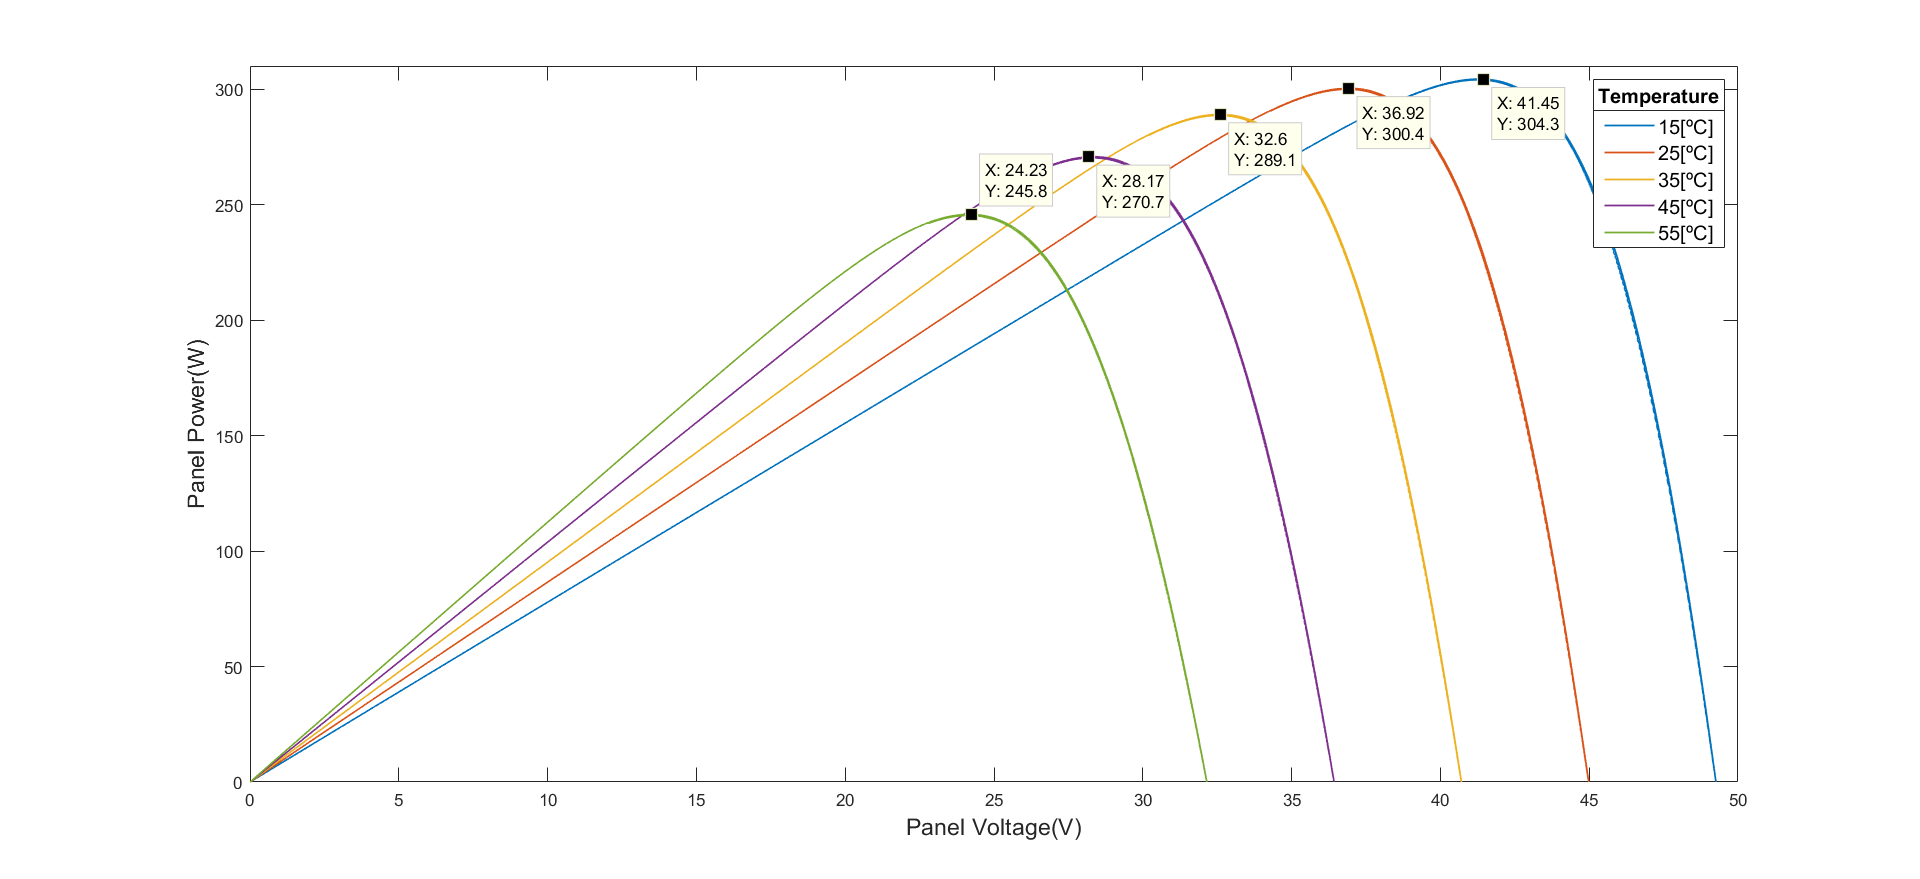
\includegraphics[width=0.83\textwidth]{../Pictures/PV_curves_1000_irradiance}
		\caption{P-V curves for constant irradiance (1000$W/ m^2$) and change in temperature.}
		\label{fig:PVcurves_Irr1000} 
	\end{center}	
\end{figure}


\begin{figure}[H]
	\begin{center}
		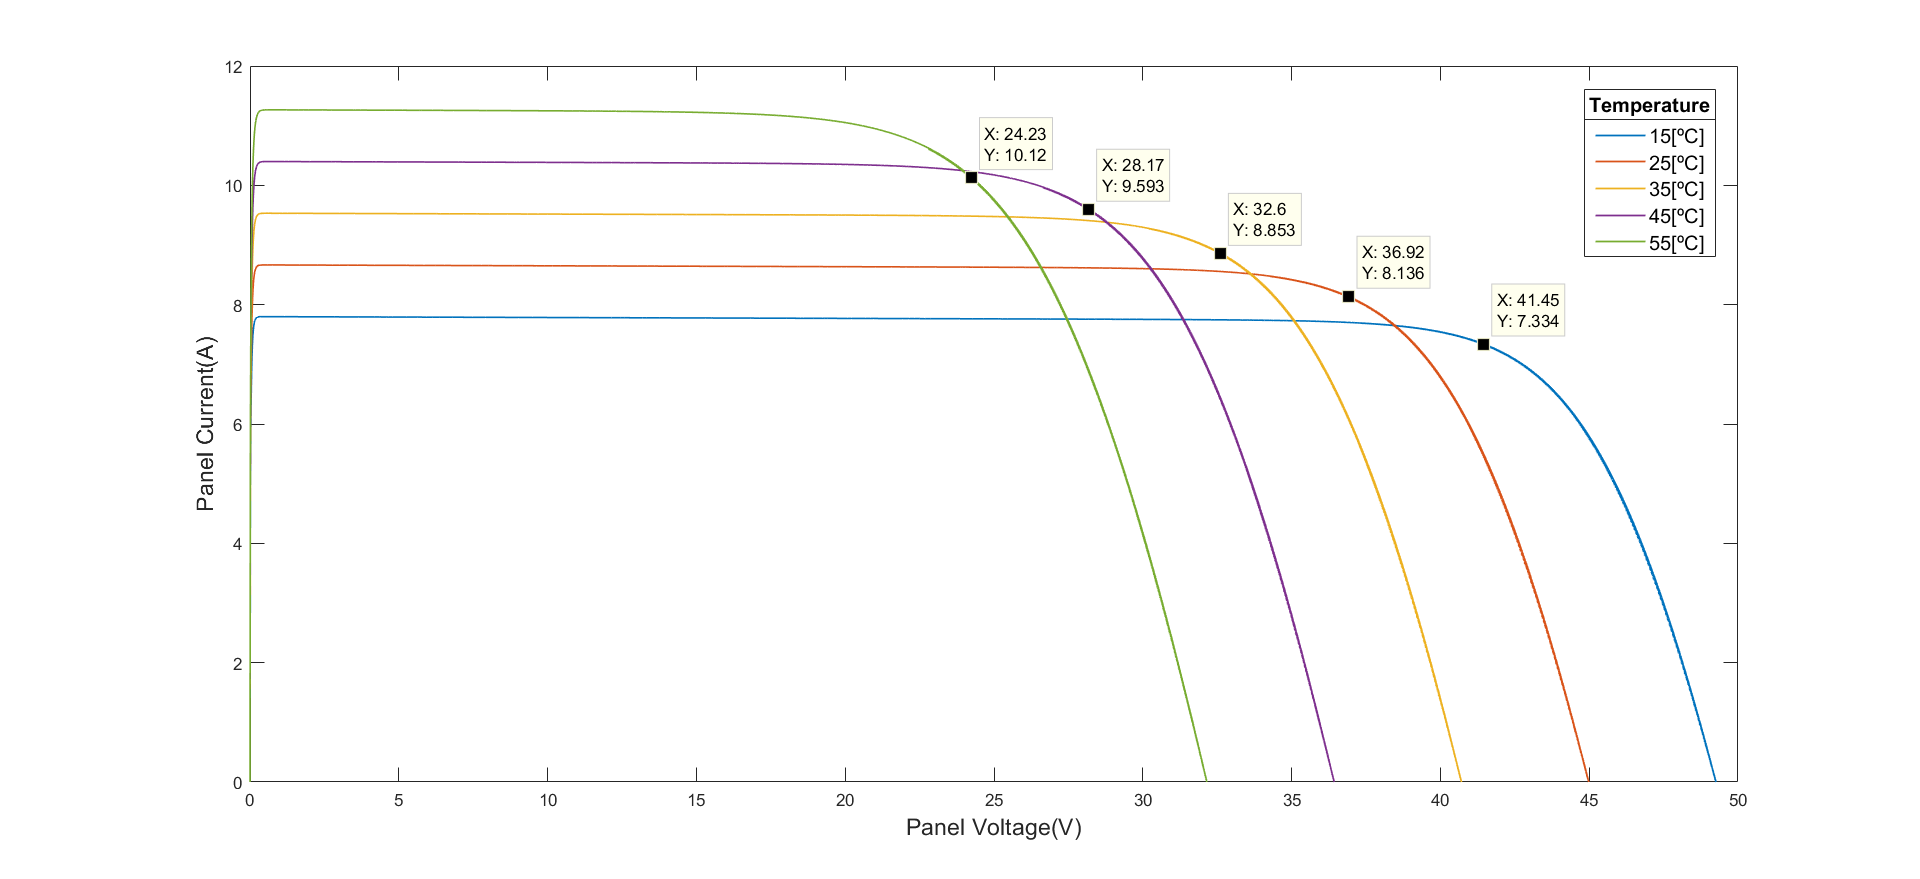
\includegraphics[width=0.83\textwidth]{../Pictures/IV_curves_1000_irradiance}
		\caption{I-V curves for constant irradiance (1000$W/ m^2$) and change in temperature.}
		\label{fig:IVcurves_Irr1000} 
	\end{center}	
\end{figure}


\subsection{MPPT algorithm results}

THINGS TO WRITE:
\begin{itemize}
	\item For each load value (buck and boost) show the grahs corresponding to change in irradiance, change in temperature 
	\item Graphs: Vin/Iin/Pin. Control variable/Dbuck/Dboost/Vinvsvout
	\item Efficiency of the MPPT in buck and boost
	
\end{itemize}
